\documentclass{beamer}

\usepackage{amsmath}
\usepackage{amssymb}
\usepackage{bm}
\usepackage[utf8]{inputenc}
\usepackage[vietnamese]{babel}
\usepackage{graphicx}
\usepackage{booktabs}

\usetheme{hust}

\title{Hợp Nhất Ảnh Y Tế}
\subtitle{Các Chỉ Số Đánh Giá Hiệu Suất Hợp Nhất Ảnh}
\author{Đỗ Trung Kiên}
\institute{Đại học Bách khoa Hà Nội}
\date{\today}

\begin{document}

% ============================================================
% Slide 1: Title
% ============================================================
\frame{\titlepage}

% ============================================================
% Slide 2: Table of Contents
% ============================================================
\begin{frame}{Nội dung trình bày}
    \tableofcontents
\end{frame}

% ============================================================
% Slide 3: Introduction
% ============================================================
\begin{frame}{Giới thiệu \& Phương pháp hợp nhất ảnh}
    Hợp nhất ảnh y tế là quá trình kết hợp thông tin từ nhiều nguồn ảnh khác nhau (các phương thức khác nhau) nhằm cải thiện chất lượng ảnh phục vụ chẩn đoán.

    \vspace{0.4cm}
    \textbf{Hai phương pháp hợp nhất ảnh chính được xem xét:}
    \begin{itemize}
        \item \textbf{Hợp nhất trực tiếp VI-IR:} Hợp nhất ảnh không đồng nhất giữa ảnh hồng ngoại (IR) và ảnh khả kiến (VI) ở cấp độ điểm ảnh.
        \item \textbf{Hợp nhất cải tiến VI-EVI:} Hợp nhất ảnh đồng nhất (ảnh khả kiến được tăng cường từ ảnh hồng ngoại sẽ được hợp nhất với ảnh khả kiến gốc).
    \end{itemize}

    \vspace{0.4cm}
    \textbf{Đánh giá hiệu suất:}
    \begin{itemize}
        \item Đánh giá có tham chiếu (Yêu cầu phải có ảnh chuẩn - Ground Truth).
        \item \textbf{Đánh giá mù (Không cần tham chiếu)} $\rightarrow$ \textit{Trọng tâm của bài nghiên cứu này}.
    \end{itemize}
\end{frame}


% ============================================================
% Slide: Demo kết quả hợp nhất ảnh (ảnh minh họa)
% ============================================================
\begin{frame}{Kết quả hợp nhất ảnh -- Minh họa}
    \begin{figure}
        \centering
        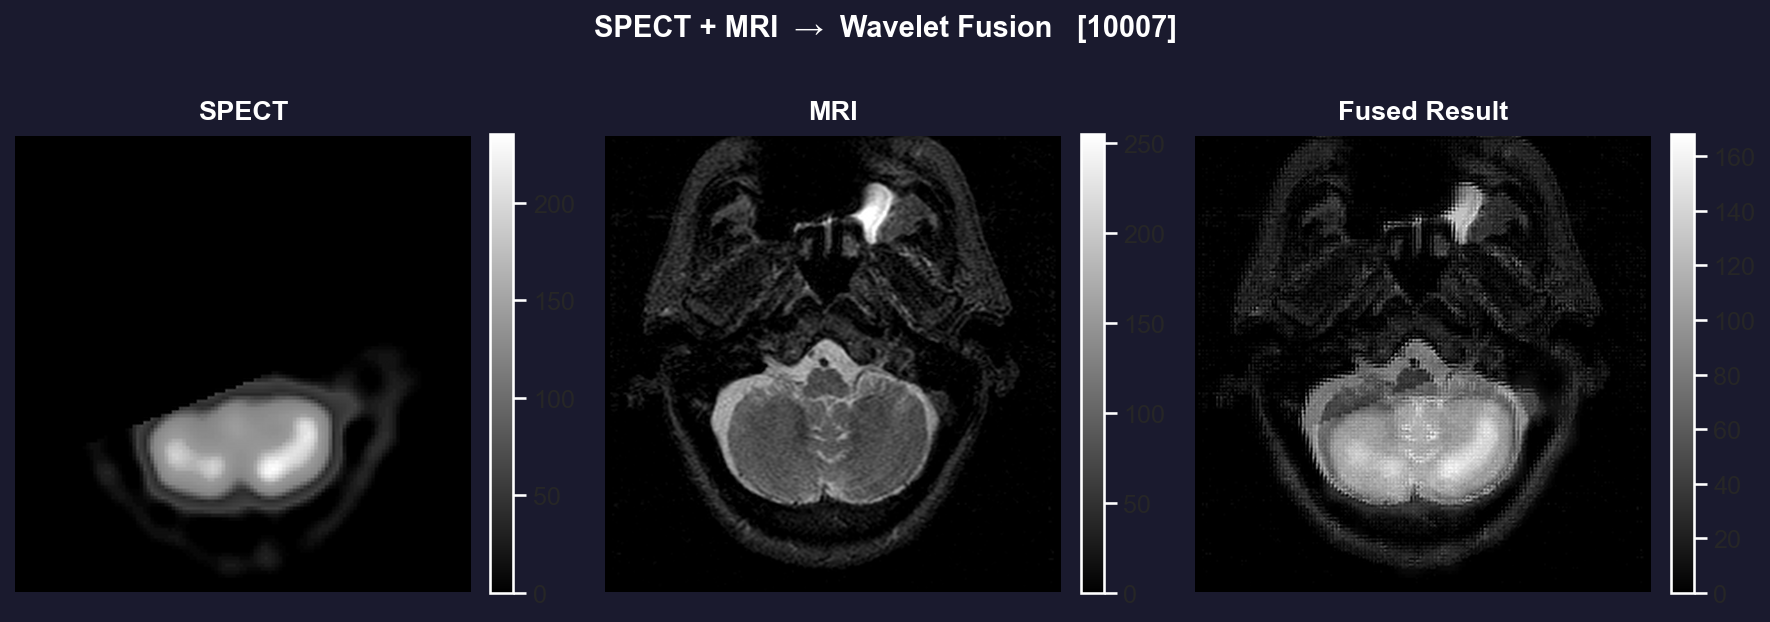
\includegraphics[width=0.92\textwidth]{Image/fusion_10007.png}
        \caption{Ví dụ 1: Ảnh nguồn A \quad|\quad Ảnh nguồn B \quad|\quad Ảnh sau hợp nhất (Wavelet Fusion)}
    \end{figure}
\end{frame}

\begin{frame}{Kết quả hợp nhất ảnh -- Minh họa (tiếp)}
    \begin{figure}
        \centering
        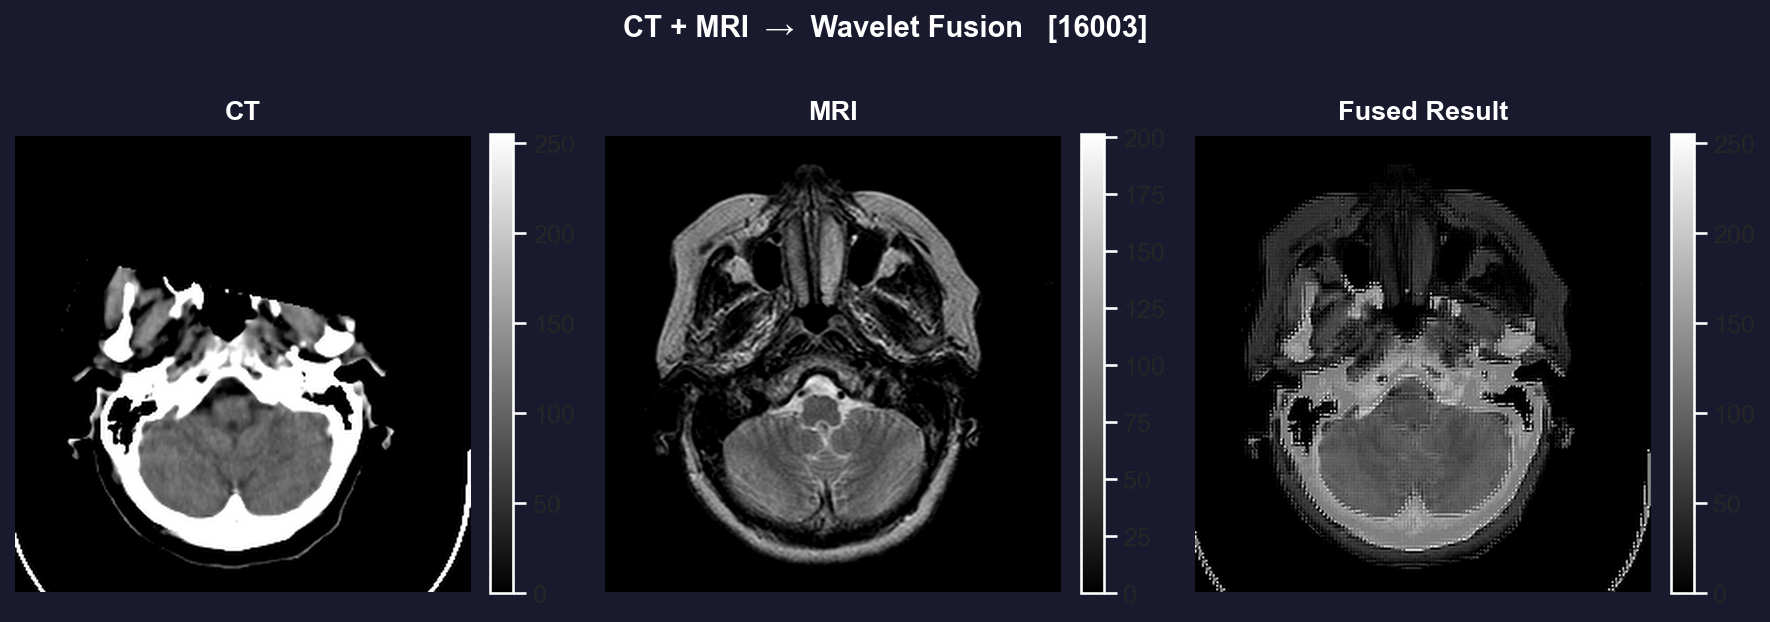
\includegraphics[width=0.92\textwidth]{Image/fusion_16003.png}
        \caption{Ví dụ 2: Ảnh nguồn A \quad|\quad Ảnh nguồn B \quad|\quad Ảnh sau hợp nhất (Wavelet Fusion)}
    \end{figure}
\end{frame}


% ============================================================
\section{Information Theory-Based Metrics}
% ============================================================

% --- Slide: QMI (Part 1) ---
\begin{frame}{1. Thông tin tương hỗ chuẩn hóa ($Q_{MI}$)}
    Thông tin tương hỗ (Mutual Information - MI) định lượng khoảng cách giữa phân phối xác suất kết hợp và phân phối biên khi các biến độc lập.

    \begin{block}{Thông tin tương hỗ (MI)}
    \begin{equation}
        MI(U,V) = \sum_{u \in U} \sum_{v \in V} p(u,v) \log_2 \frac{p(u,v)}{p(u)p(v)}
    \end{equation}
    \end{block}

    Tương đương, MI có thể được biểu diễn thông qua entropy kết hợp $H(U,V)$ và các entropy biên $H(U), H(V)$:
    \begin{equation}
        MI(U,V) = H(U) + H(V) - H(U,V)
    \end{equation}
\end{frame}

% --- Slide: QMI (Part 2) ---
\begin{frame}{1. Thông tin tương hỗ chuẩn hóa ($Q_{MI}$)}
    Đối với các ảnh đầu vào $A, B$ và ảnh sau khi hợp nhất $F$:

    \vspace{0.3cm}
    \textbf{Thước đo của Qu và cộng sự:}
    \begin{equation}
        M_{F}^{AB} = MI(A,F) + MI(B,F)
    \end{equation}
    \textit{Nhược điểm:} Việc kết hợp các entropy ở các thang đo khác nhau có thể gây mất ổn định và làm sai lệch thước đo.

    \vspace{0.3cm}
    \textbf{Thước đo của Hossny (Được sử dụng trong nghiên cứu):}
    \begin{block}{$Q_{MI}$ chuẩn hóa}
    \begin{equation}
        Q_{MI} = 2 \left[ \frac{MI(A,F)}{H(A)+H(F)} + \frac{MI(B,F)}{H(B)+H(F)} \right]
    \end{equation}
    \end{block}
\end{frame}

% --- Slide: QTE ---
\begin{frame}{2. Thước đo dựa trên Entropy Tsallis ($Q_{TE}$)}
    Entropy Tsallis là phép đo sự phân kỳ về mức độ phụ thuộc giữa hai biến ngẫu nhiên rời rạc.

    \begin{block}{Entropy Tsallis ($q \neq 1$)}
    \begin{equation}
        I_q(A,F) = \frac{1}{1-q} \sum_{i,j} \left( \frac{h_{AF}(i,j)^q}{h_F(j)h_A(i)^{q-1}} \right)
    \end{equation}
    \end{block}

    \textbf{Thước đo Tsallis chuẩn hóa (Nava và cộng sự):}
    \begin{equation}
        Q_{TE} = \frac{I_q(A,F) + I_q(B,F)}{H_q(A) + H_q(B) - I_q(A,B)}
    \end{equation}

    \vspace{0.2cm}
    \footnotesize{\textit{Lưu ý: Các phương pháp dựa trên MI thường nhạy cảm với nhiễu xung và nhiễu Gaussian, do đó $Q_{TE}$ được đề xuất như một giải pháp thay thế mạnh mẽ và ổn định hơn.}}
\end{frame}

% --- Slide: QNCIE (Part 1) ---
\begin{frame}{3. Entropy thông tin tương quan phi tuyến ($Q_{NCIE}$)}
    \textbf{Hệ số tương quan phi tuyến (NCC):}
    \begin{equation}
        NCC(U,V) = H^b(U) + H^b(V) - H^b(U,V)
    \end{equation}
    Trong đó $b=256$ (số mức xám của ảnh), và các entropy được tính bằng:
    $H^b(A) = \sum h_A(i)\log_b h_A(i)$.

    \vspace{0.3cm}
    \textbf{Ma trận tương quan phi tuyến ($R$):}
    \begin{equation}
        R = \begin{bmatrix}
            1 & NCC_{AB} & NCC_{AF} \\
            NCC_{BA} & 1 & NCC_{BF} \\
            NCC_{FA} & NCC_{FB} & 1
        \end{bmatrix}
    \end{equation}
\end{frame}

% --- Slide: QNCIE (Part 2) ---
\begin{frame}{3. Entropy thông tin tương quan phi tuyến ($Q_{NCIE}$)}
    Gọi $\lambda_i$ (với $i=1, 2, 3$) là các giá trị riêng (eigenvalues) của ma trận tương quan phi tuyến $R$.

    \vspace{0.5cm}
    Giá trị của Entropy thông tin tương quan phi tuyến ($Q_{NCIE}$) được xác định bởi công thức:

    \begin{block}{Thước đo $Q_{NCIE}$}
    \begin{equation}
        Q_{NCIE} = 1 + \sum_{i=1}^3 \frac{\lambda_i}{3} \log_b \frac{\lambda_i}{3}
    \end{equation}
    \end{block}
\end{frame}


% ============================================================
\section{Image Feature-Based Metrics}
% ============================================================

% --- Slide: QG (Gradient) ---
\begin{frame}{4. Thước đo dựa trên Gradient ($Q_G$)}
    Đề xuất bởi Xydeas và Petrovic, thước đo này đánh giá lượng \textbf{thông tin cạnh (edge information)} được truyền từ ảnh đầu vào sang ảnh trộn, sử dụng toán tử Sobel.

    \vspace{0.2cm}
    Cường độ biên $g_A(i,j)$ và hướng biên $\alpha_A(i,j)$ của ảnh $A$:
    \begin{equation}
        g_A(i,j) = \sqrt{s^x_A(i,j)^2 + s^y_A(i,j)^2}, \quad \alpha_A(i,j) = \arctan \left( \frac{s^x_A(i,j)}{s^y_A(i,j)} \right)
    \end{equation}

    \vspace{0.2cm}
    Tổng hợp giá trị bảo toàn thông tin cạnh $Q^{AF}(i,j)$ và $Q^{BF}(i,j)$, ta có thước đo tổng thể:
    \begin{block}{Thước đo $Q_G$}
    \begin{equation}
        Q_G = \frac{\sum_{i=1}^N \sum_{j=1}^M \left[ Q^{AF}(i,j)w_A(i,j) + Q^{BF}(i,j)w_B(i,j) \right]}{\sum_{i=1}^N \sum_{j=1}^M \left[ w_A(i,j) + w_B(i,j) \right]}
    \end{equation}
    \end{block}
    \footnotesize{\textit{Trong đó $w_A, w_B$ là các trọng số phụ thuộc vào cường độ biên.}}
\end{frame}

% --- Slide: QM (Multiscale) ---
\begin{frame}{5. Thước đo đa tỷ lệ ($Q_M$)}
    Đề xuất bởi Wang và Liu, sử dụng phân tích \textbf{Wavelet Haar 2 cấp}. Thông tin cạnh được trích xuất từ các thành phần tần số cao (ngang, dọc, chéo).

    \vspace{0.2cm}
    Giá trị bảo toàn cạnh toàn cục tại tỷ lệ $s$:
    \begin{equation}
        EP^{AF}_s = \frac{\Delta^{AF}_{Hs} + \Delta^{AF}_{Vs} + \Delta^{AF}_{Ds}}{3}
    \end{equation}

    Thước đo chuẩn hóa tại tỷ lệ $s$ ($Q_s^{AB/F}$) được tính bằng trung bình có trọng số, với trọng số $w$ là năng lượng tần số cao của ảnh gốc.

    \begin{block}{Thước đo $Q_M$ tổng thể}
    \begin{equation}
        Q_M = \prod_{s=1}^N \left( Q_s^{AB/F} \right)^{\alpha_s}
    \end{equation}
    \end{block}
    \footnotesize{\textit{$\alpha_s$ là hằng số điều chỉnh tầm quan trọng của các mức tỷ lệ khác nhau.}}
\end{frame}

% --- Slide: QSF (Spatial Frequency) ---
\begin{frame}{6. Thước đo Tần số không gian ($Q_{SF}$)}
    Zheng và cộng sự sử dụng ``Tần số không gian'' (Spatial Frequency - SF) để đo lường \textbf{mức độ hoạt động (activity level)} của một bức ảnh.

    \begin{equation}
        SF = \sqrt{RF^2 + CF^2 + MDF^2 + SDF^2}
    \end{equation}
    Trong đó:
    \begin{itemize}
        \item $RF, CF$: Gradient theo hướng ngang (Row) và dọc (Column).
        \item $MDF, SDF$: Gradient theo đường chéo chính và chéo phụ (kèm trọng số khoảng cách $w_d = 1/\sqrt{2}$).
    \end{itemize}

    \begin{block}{Thước đo $Q_{SF}$}
    \begin{equation}
        Q_{SF} = \frac{SF_F - SF_R}{SF_R}
    \end{equation}
    \end{block}
    \footnotesize{\textit{$SF_F$ là tần số không gian của ảnh trộn, $SF_R$ là tần số không gian tham chiếu (lấy max gradient từ ảnh A và B).}}
\end{frame}

% --- Slide: QP (Phase Congruency) ---
\begin{frame}{7. Thước đo dựa trên Đồng pha ($Q_P$)}
    Zhao và Liu sử dụng tính đồng pha (Phase Congruency), cung cấp phép đo \textbf{tuyệt đối về đặc trưng ảnh} (như góc, cạnh) bất chấp độ tương phản.

    Thước đo là tích của 3 hệ số tương quan dựa trên momen của đồng pha:
    \begin{block}{Thước đo $Q_P$}
    \begin{equation}
        Q_P = (P_p)^\alpha (P_M)^\beta (P_m)^\gamma
    \end{equation}
    \end{block}

    \begin{itemize}
        \item $P_p$: Giá trị đồng pha (phase congruency).
        \item $P_M, P_m$: Momen chính cực đại (Maximum) và cực tiểu (Minimum), chứa thông tin về các góc và cạnh.
        \item $\alpha, \beta, \gamma$: Các tham số hàm mũ điều chỉnh tầm quan trọng của 3 thành phần.
    \end{itemize}
\end{frame}


% ============================================================
\section{Image Structural Similarity-Based Metrics}
% ============================================================

% --- Slide: SSIM & UIQI ---
\begin{frame}{8. Độ tương đồng cấu trúc (SSIM \& UIQI)}
    Hệ thống thị giác của con người rất nhạy cảm với thông tin cấu trúc. Wang đã đề xuất chỉ số \textbf{SSIM} dựa trên 3 thành phần: Độ sáng ($l$), Độ tương phản ($c$) và Độ tương quan ($s$).

    \begin{block}{Chỉ số SSIM}
    \begin{equation}
        SSIM(A,B) = \frac{(2\mu_A\mu_B + C_1)(2\sigma_{AB} + C_2)}{(\mu_A^2 + \mu_B^2 + C_1)(\sigma_A^2 + \sigma_B^2 + C_2)}
    \end{equation}
    \end{block}
    \textit{Trong đó: $\mu$ là giá trị trung bình, $\sigma^2$ là phương sai, $\sigma_{AB}$ là hiệp phương sai. $C_1, C_2$ là hằng số chống chia cho 0.}

    \vspace{0.3cm}
    Khi $C_1 = C_2 = 0$, SSIM trở thành \textbf{Chỉ số chất lượng ảnh phổ quát (UIQI - $Q$)}:
    \begin{equation}
        Q(A,B) = \frac{4\sigma_{AB}\mu_A\mu_B}{(\sigma_A^2 + \sigma_B^2)(\mu_A^2 + \mu_B^2)}
    \end{equation}
\end{frame}

% --- Slide: SSIM-based Variants ---
\begin{frame}{9. Các biến thể dựa trên SSIM (Cửa sổ trượt)}
    Thay vì tính trên toàn bộ ảnh, các tác giả đề xuất sử dụng phương pháp \textbf{cửa sổ trượt (sliding window - $w$)} để đánh giá cục bộ:

    \begin{itemize}
        \item \textbf{Thước đo của Piella ($Q_S, Q_W, Q_E$):} Kết hợp UIQI cục bộ với trọng số $\lambda(w)$ dựa trên độ nổi bật (phương sai) của khu vực ảnh.
        \item \textbf{Thước đo của Cvejie ($Q_C$):} Trọng số phụ thuộc vào độ tương đồng không gian giữa ảnh đầu vào và ảnh trộn.
        \item \textbf{Thước đo của Yang ($Q_Y$):} Sử dụng hàm điều kiện dựa trên mức độ tương đồng cục bộ:
    \end{itemize}

    \begin{equation}
    Q_Y =
    \begin{cases}
      \lambda(w) SSIM_A + (1-\lambda(w)) SSIM_B & \text{nếu } SSIM(A,B|w) \ge 0.75 \\
      \max \{SSIM_A, SSIM_B\} & \text{nếu } SSIM(A,B|w) < 0.75
   \end{cases}
   \end{equation}
\end{frame}


% ============================================================
\section{Human Perception-Inspired Fusion Metrics}
% ============================================================

% --- Slide: QCV ---
\begin{frame}{10. Thước đo Chen-Varshney ($Q_{CV}$)}
    Mô phỏng \textbf{cảm nhận thị giác con người (Human Perception)} thông qua Hàm độ nhạy tương phản (Contrast Sensitive Function - CSF). Gồm 5 bước:
    \begin{enumerate}
        \item Trích xuất thông tin cạnh (Toán tử Sobel).
        \item Chia ảnh thành các vùng cục bộ (windows).
        \item Tính độ nổi bật vùng cục bộ ($\lambda$).
        \item \textbf{Đo độ tương đồng:} Tính sai số bình phương trung bình của ảnh đã qua bộ lọc CSF ($D_A, D_B$).
        \item \textbf{Đánh giá toàn cục:} Trung bình có trọng số của các vùng:
    \end{enumerate}

    \begin{block}{Thước đo $Q_{CV}$}
    \begin{equation}
        Q_{CV} = \frac{\sum_{l=1}^L \left( \lambda_A^l D_A^l + \lambda_B^l D_B^l \right)}{\sum_{l=1}^L \left( \lambda_A^l + \lambda_B^l \right)}
    \end{equation}
    \end{block}
\end{frame}

% --- Slide: QCB ---
\begin{frame}{11. Thước đo Chen-Blum ($Q_{CB}$)}
    Mở rộng việc sử dụng bộ lọc CSF trong \textbf{miền tần số} và xem xét hiệu ứng che lấp (masking effect) của mắt người. Gồm 5 bước:
    \begin{enumerate}
        \item Lọc độ nhạy tương phản (CSF) trong miền tần số.
        \item Tính toán độ tương phản cục bộ (Peli's contrast).
        \item Tính toán bản đồ độ tương phản bị che lấp (Masked contrast map - $C'_A, C'_B$).
        \item Tạo bản đồ độ nổi bật (Saliency map - $\lambda_A, \lambda_B$).
        \item Tính bản đồ chất lượng toàn cục ($Q_{GQM}$):
    \end{enumerate}

    \begin{equation}
        Q_{GQM}(i,j) = \lambda_A(i,j)Q_{AF}(i,j) + \lambda_B(i,j)Q_{BF}(i,j)
    \end{equation}
    \textit{Thước đo $Q_{CB}$ cuối cùng là giá trị trung bình của bản đồ $Q_{GQM}$.}
\end{frame}


% ============================================================
% Slide: Kết quả số liệu
% ============================================================
\section{Result}

\begin{frame}{Kết quả đánh giá -- Bảng số liệu (1)}
    \begin{figure}
        \centering
        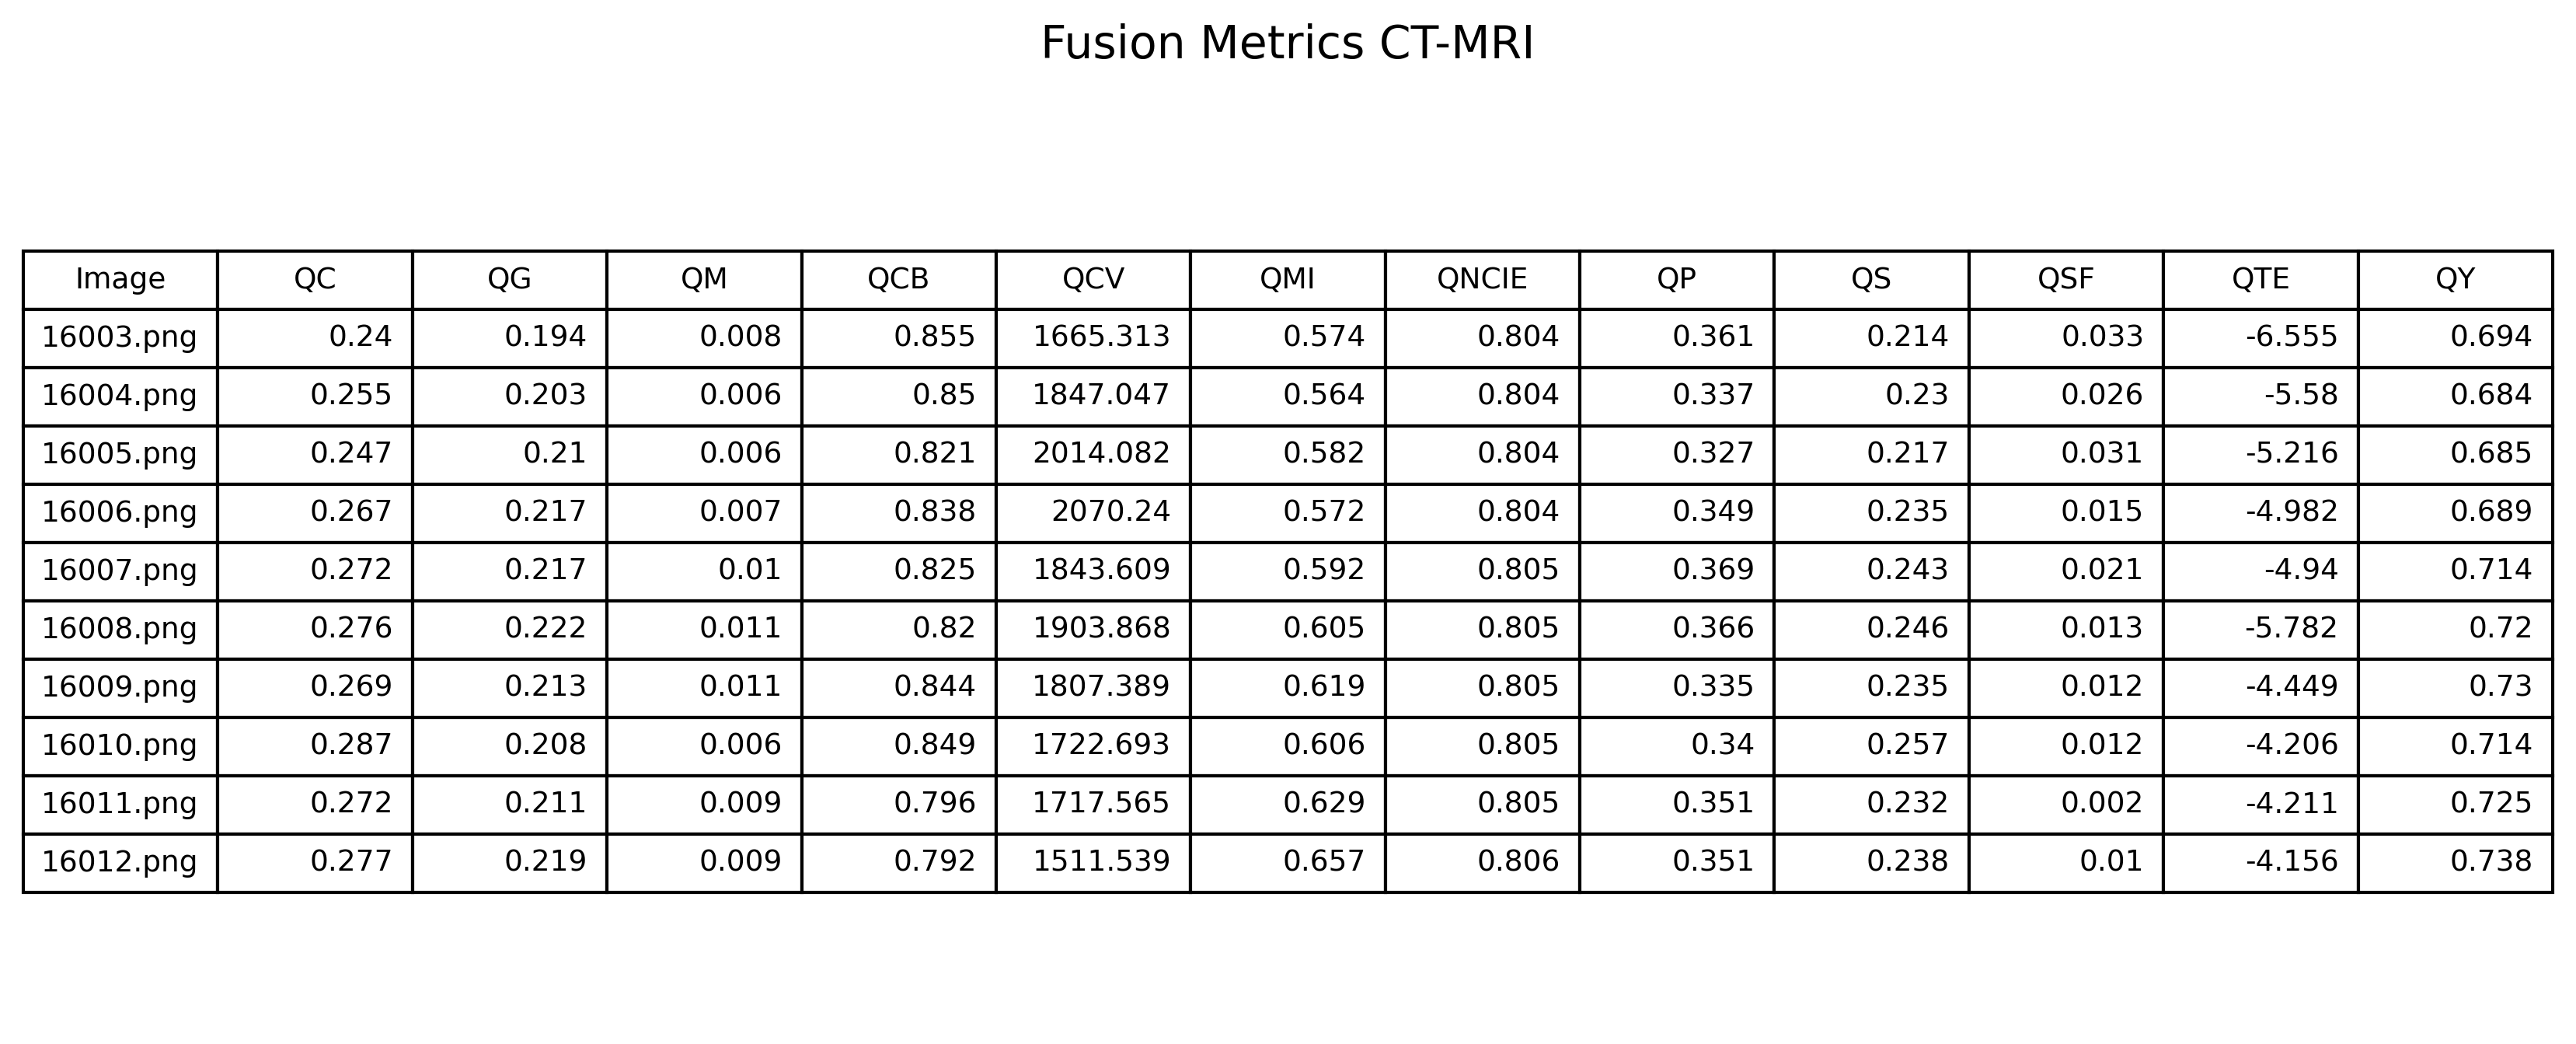
\includegraphics[width=0.95\textwidth]{Image/ct_mri_metrics.png}
        \caption{Giá trị các chỉ số đánh giá trên từng ảnh (phần 1)}
    \end{figure}
\end{frame}

\begin{frame}{Kết quả đánh giá -- Bảng số liệu (2)}
    \begin{figure}
        \centering
        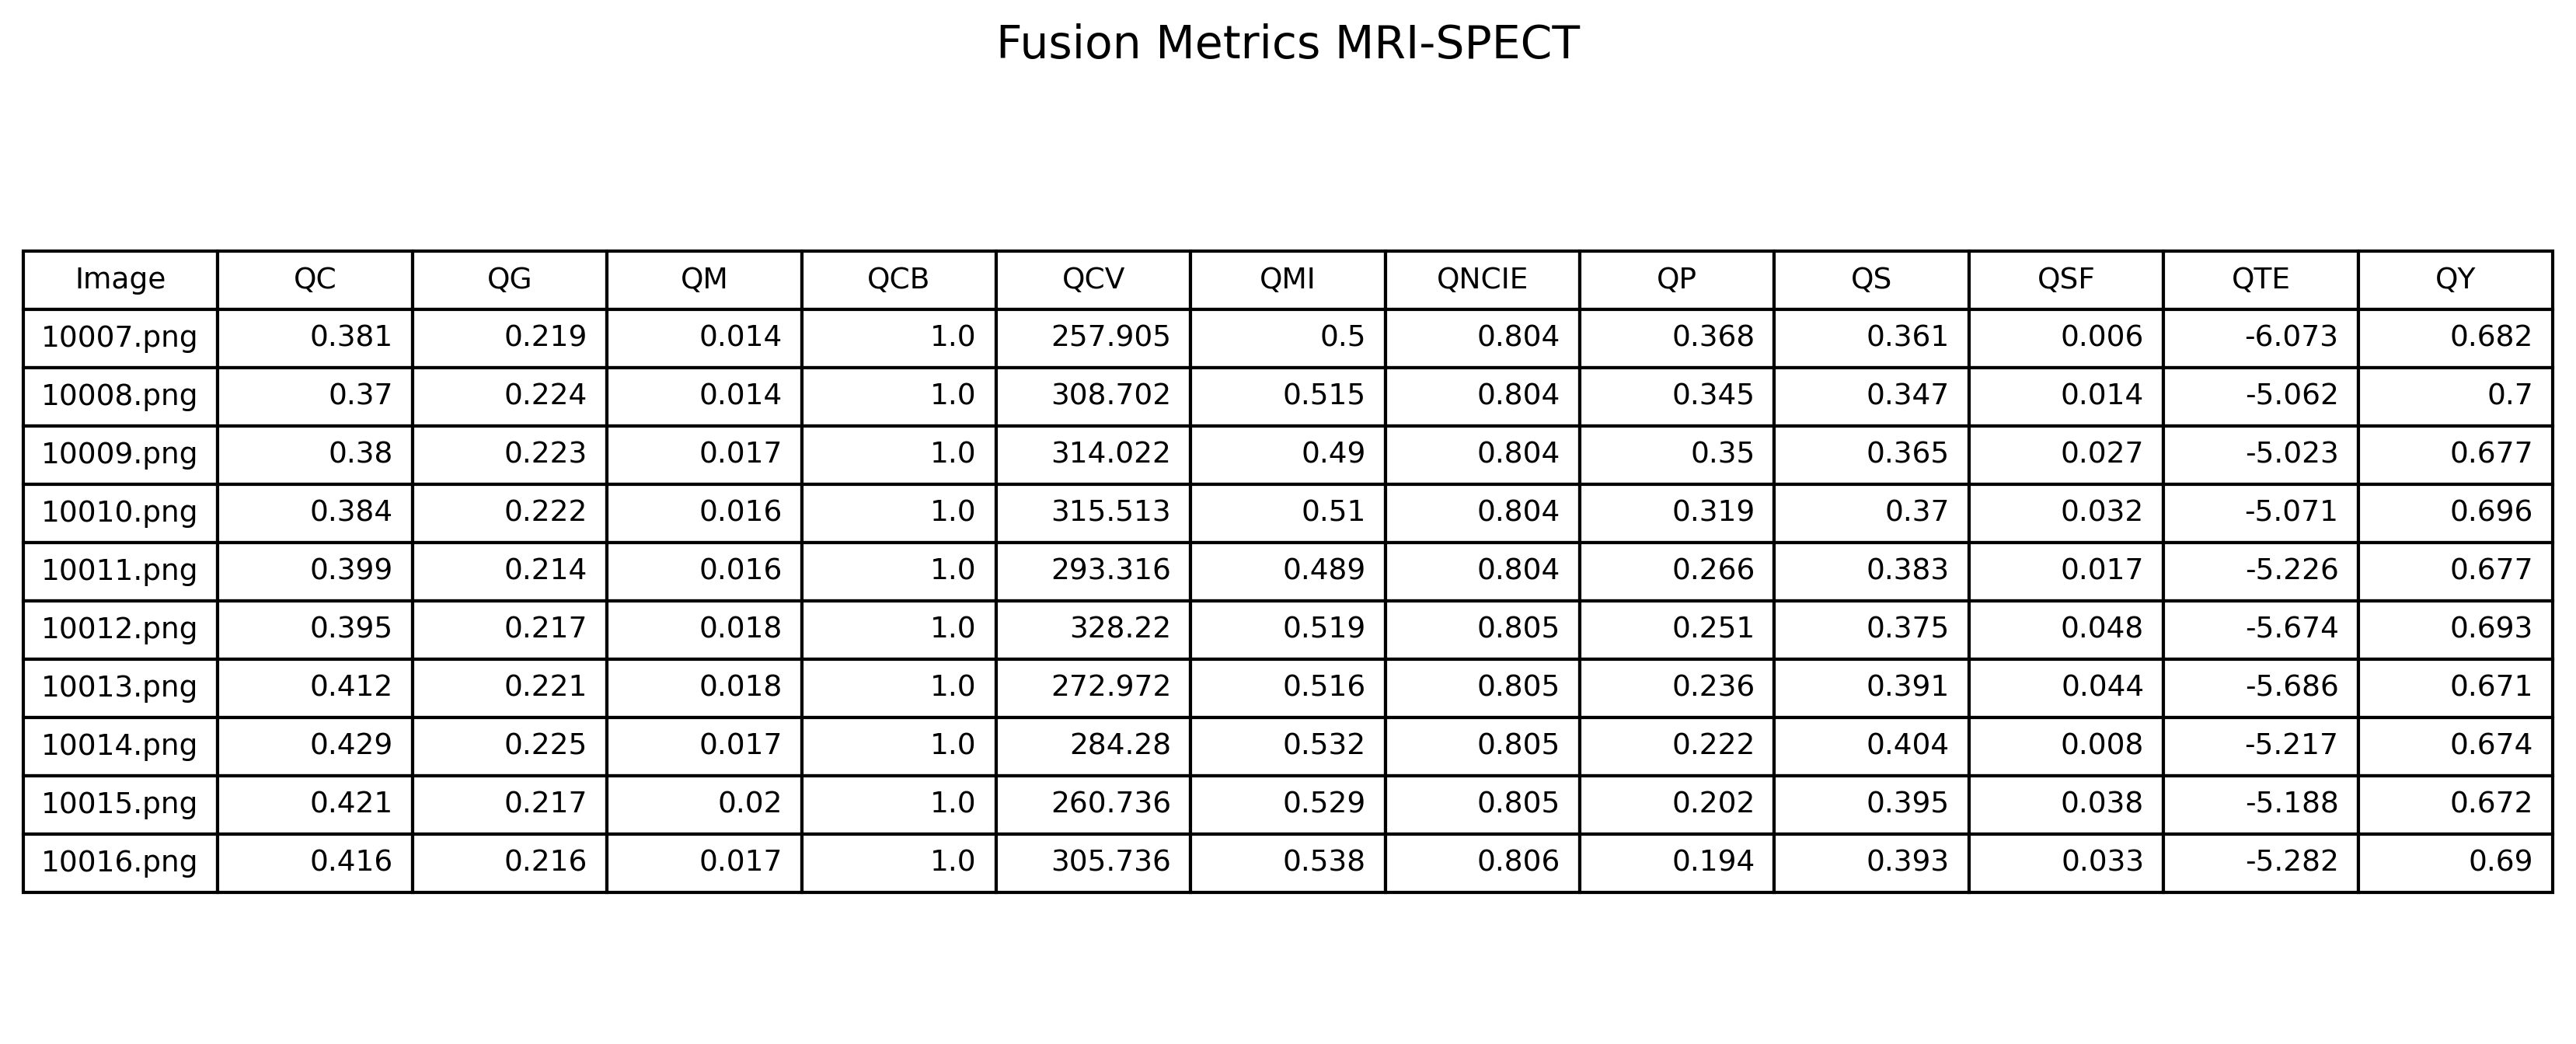
\includegraphics[width=0.95\textwidth]{Image/mri_spect_metrics.png}
        \caption{Giá trị trung bình các chỉ số đánh giá (phần 2)}
    \end{figure}
\end{frame}


% ============================================================
% Slide: Tổng kết
% ============================================================
\begin{frame}{Tổng kết}
    \begin{itemize}
        \item Đánh giá mù (không cần tham chiếu) là phương pháp rất quan trọng trong thực tế khi chúng ta không có sẵn ảnh gốc (ground truth).
        \item \textbf{11 thước đo} đã được trình bày theo 4 nhóm:
        \begin{enumerate}
            \item \textit{Information Theory-Based:} $Q_{MI}$, $Q_{TE}$, $Q_{NCIE}$
            \item \textit{Image Feature-Based:} $Q_G$, $Q_M$, $Q_{SF}$, $Q_P$
            \item \textit{Structural Similarity-Based:} SSIM/UIQI, $Q_S/Q_W/Q_E$, $Q_C$, $Q_Y$
            \item \textit{Human Perception-Inspired:} $Q_{CV}$, $Q_{CB}$
        \end{enumerate}
        \item Các thước đo toán học này cung cấp cơ sở vững chắc để đánh giá một cách khách quan chất lượng của ảnh sau khi hợp nhất.
    \end{itemize}
\end{frame}

\end{document}